\begin{solution}
\begin{enumerate}[label = \arabic*)]
    \item The file \textit{SPY\_HF.csv} contains 1-minute returns from 1993-2023 for the S\&P 500 ETF. I use the log returns to study the volatility of the series. Returns greater than 0.002 are removed to avoid data issues and outliers.\footnote{This corresponds to approximately 2\% of the entire sample} Given a sampling frequency, I cumulate the returns to upsample our series to the desired frequency and then use this series to compute the realized volatility measure. 

    For the sampling frequency, I use a sequence from 1 to 60 minutes with a step of 1 minute. As seen in the lecture notes, the volatility estimator tends to diverge as \(\Delta \to 0\) as the microstructure noise in the data starts to dominate in very high frequencies. This is exemplified in Figure~\ref{fig:volatility_signature}. This figure plots the average daily volatility as a function of the sampling frequency as well as an exponential trend. We can see that the volatility is approximately constant for frequencies between 1 and 20 minutes and it starts to exponentially rise due to the microstructure noise.

    \begin{figure}[!htbp]
        \centering
        \caption{Volatility Signature Plot}
        \label{fig:volatility_signature}
        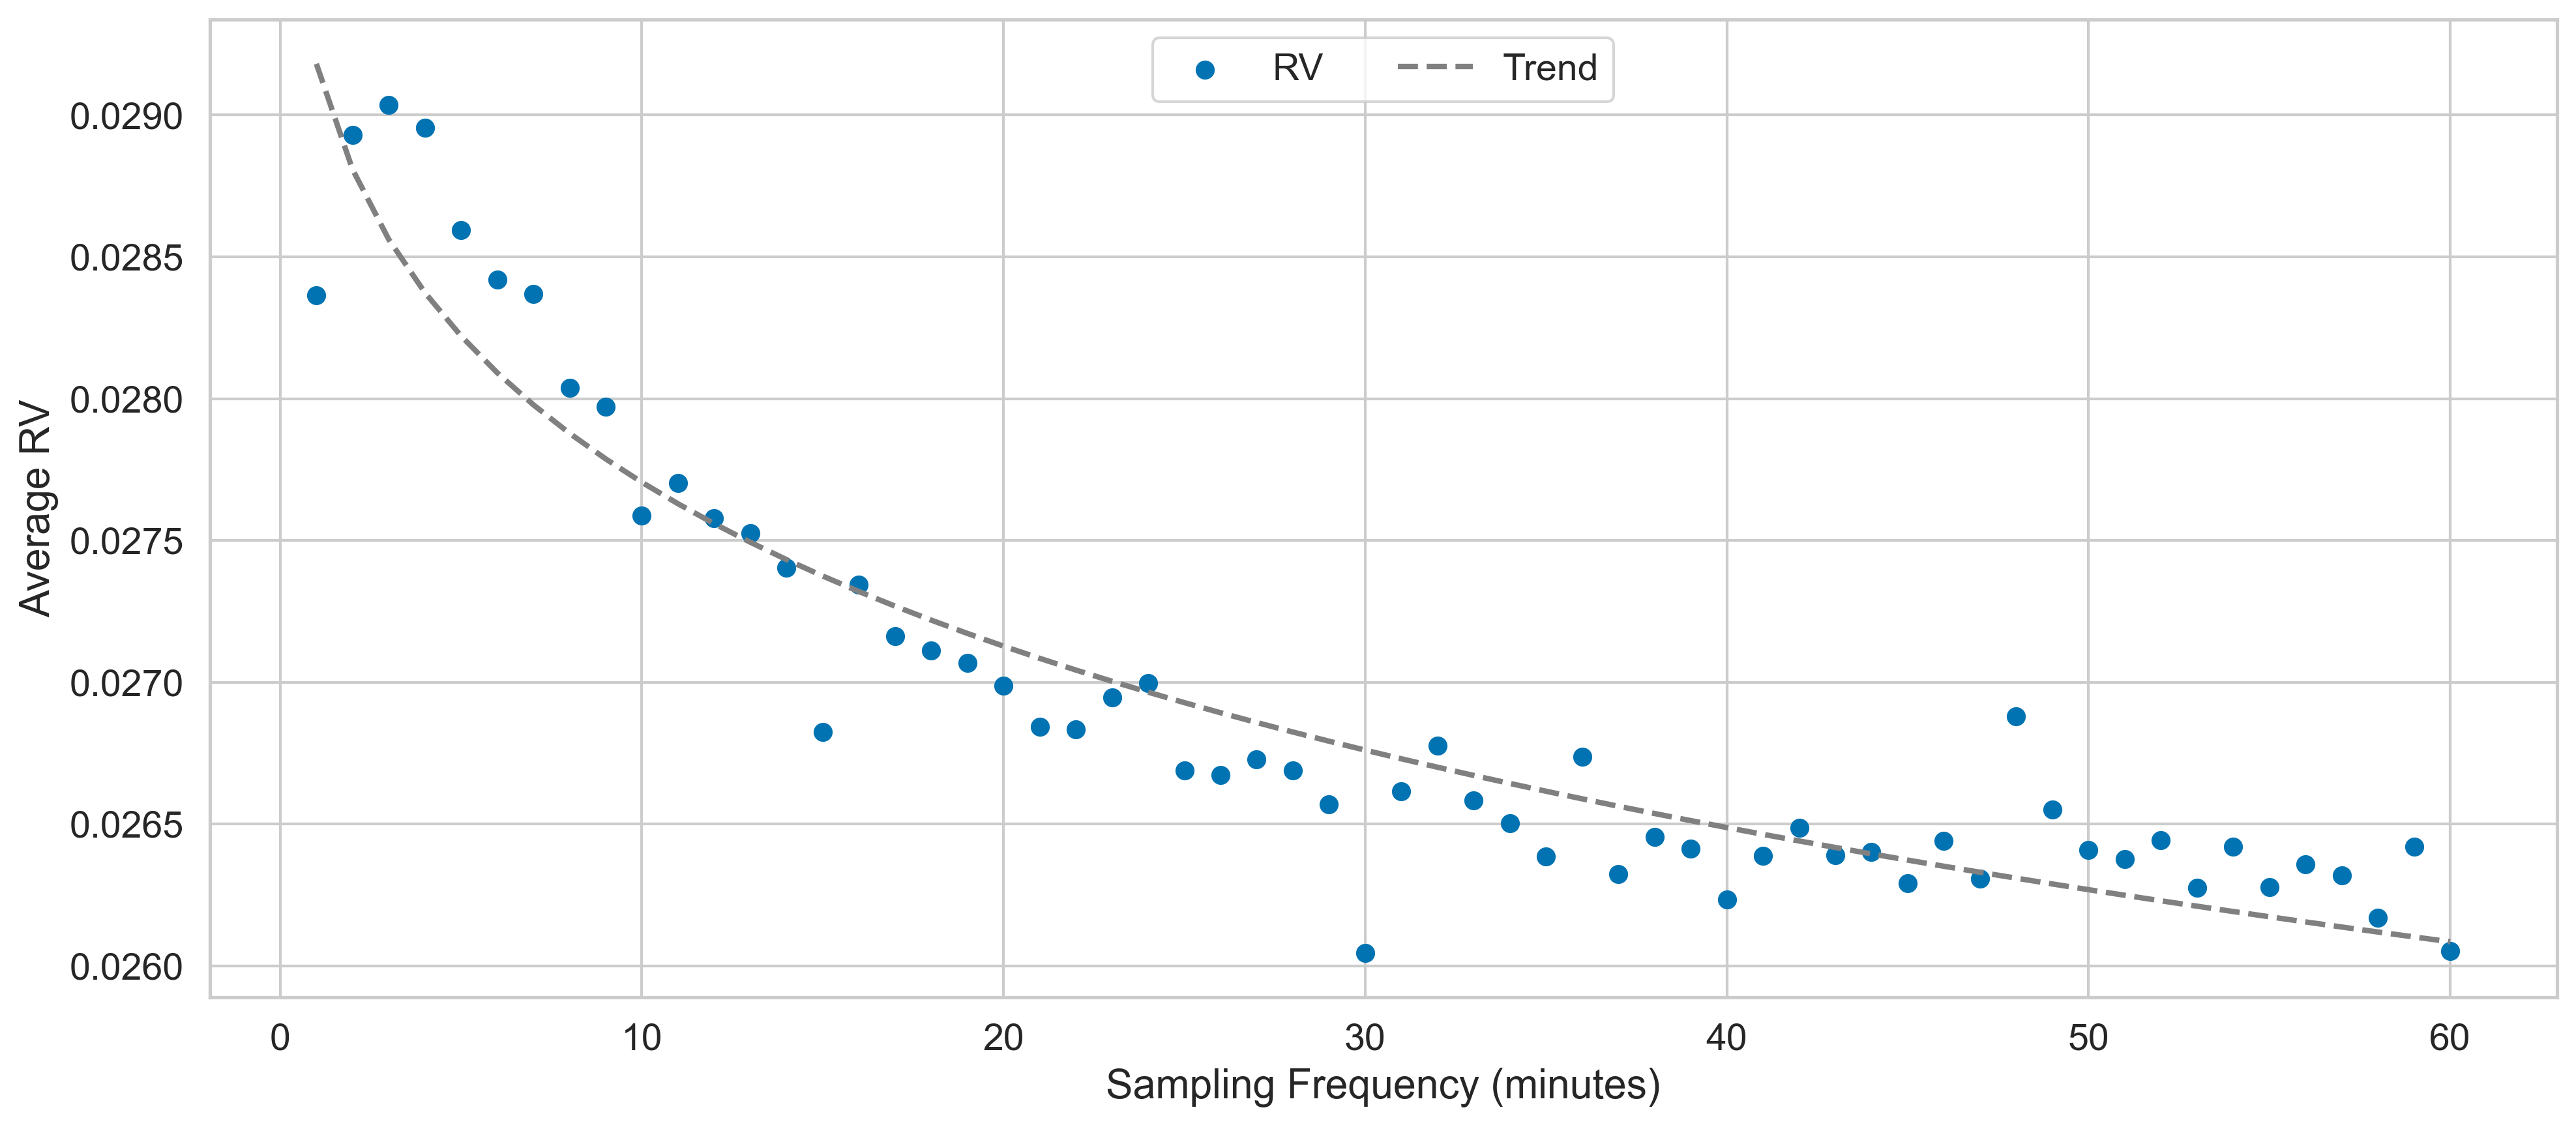
\includegraphics[width=.8\textwidth]{volatility_signature.png}
    \end{figure}
    
    \item This question will study the U-shape pattern of volatility. This phenomenom states that the market volatility is higher in the first and last hours of the trading day, and lower in the middle of the day. This is due to the fact that the market is more active in the first and last hours of the day, and less active in the middle of the day. 

    To understand this, I group the observations by the minute of the day and compute the average absolute return for each of these minutes. The NYSE TAQ database follows the Eastern Time Zone. So market hours are from 9:30 to 16:00. The first minutes of the trading day display very high noise due to the high inflow of information in the overnight. For this reason, I exclude the first 30 minutes in my analysis and only consider the information starting at 10am. 
    
    The results are shown in Figure~\ref{fig:volatility_smile}. We can see that the volatility is higher in the first and last hours of the day, and lower in the middle of the day. This is consistent with the volatility smile stylized fact. Moreover, they seem to exhibit some seasonality, with the volatility spiking up at every 30 minutes. 

    \begin{figure}[!htbp]
        \centering
        \caption{Intraday Volatility Pattern}
        \label{fig:volatility_smile}
        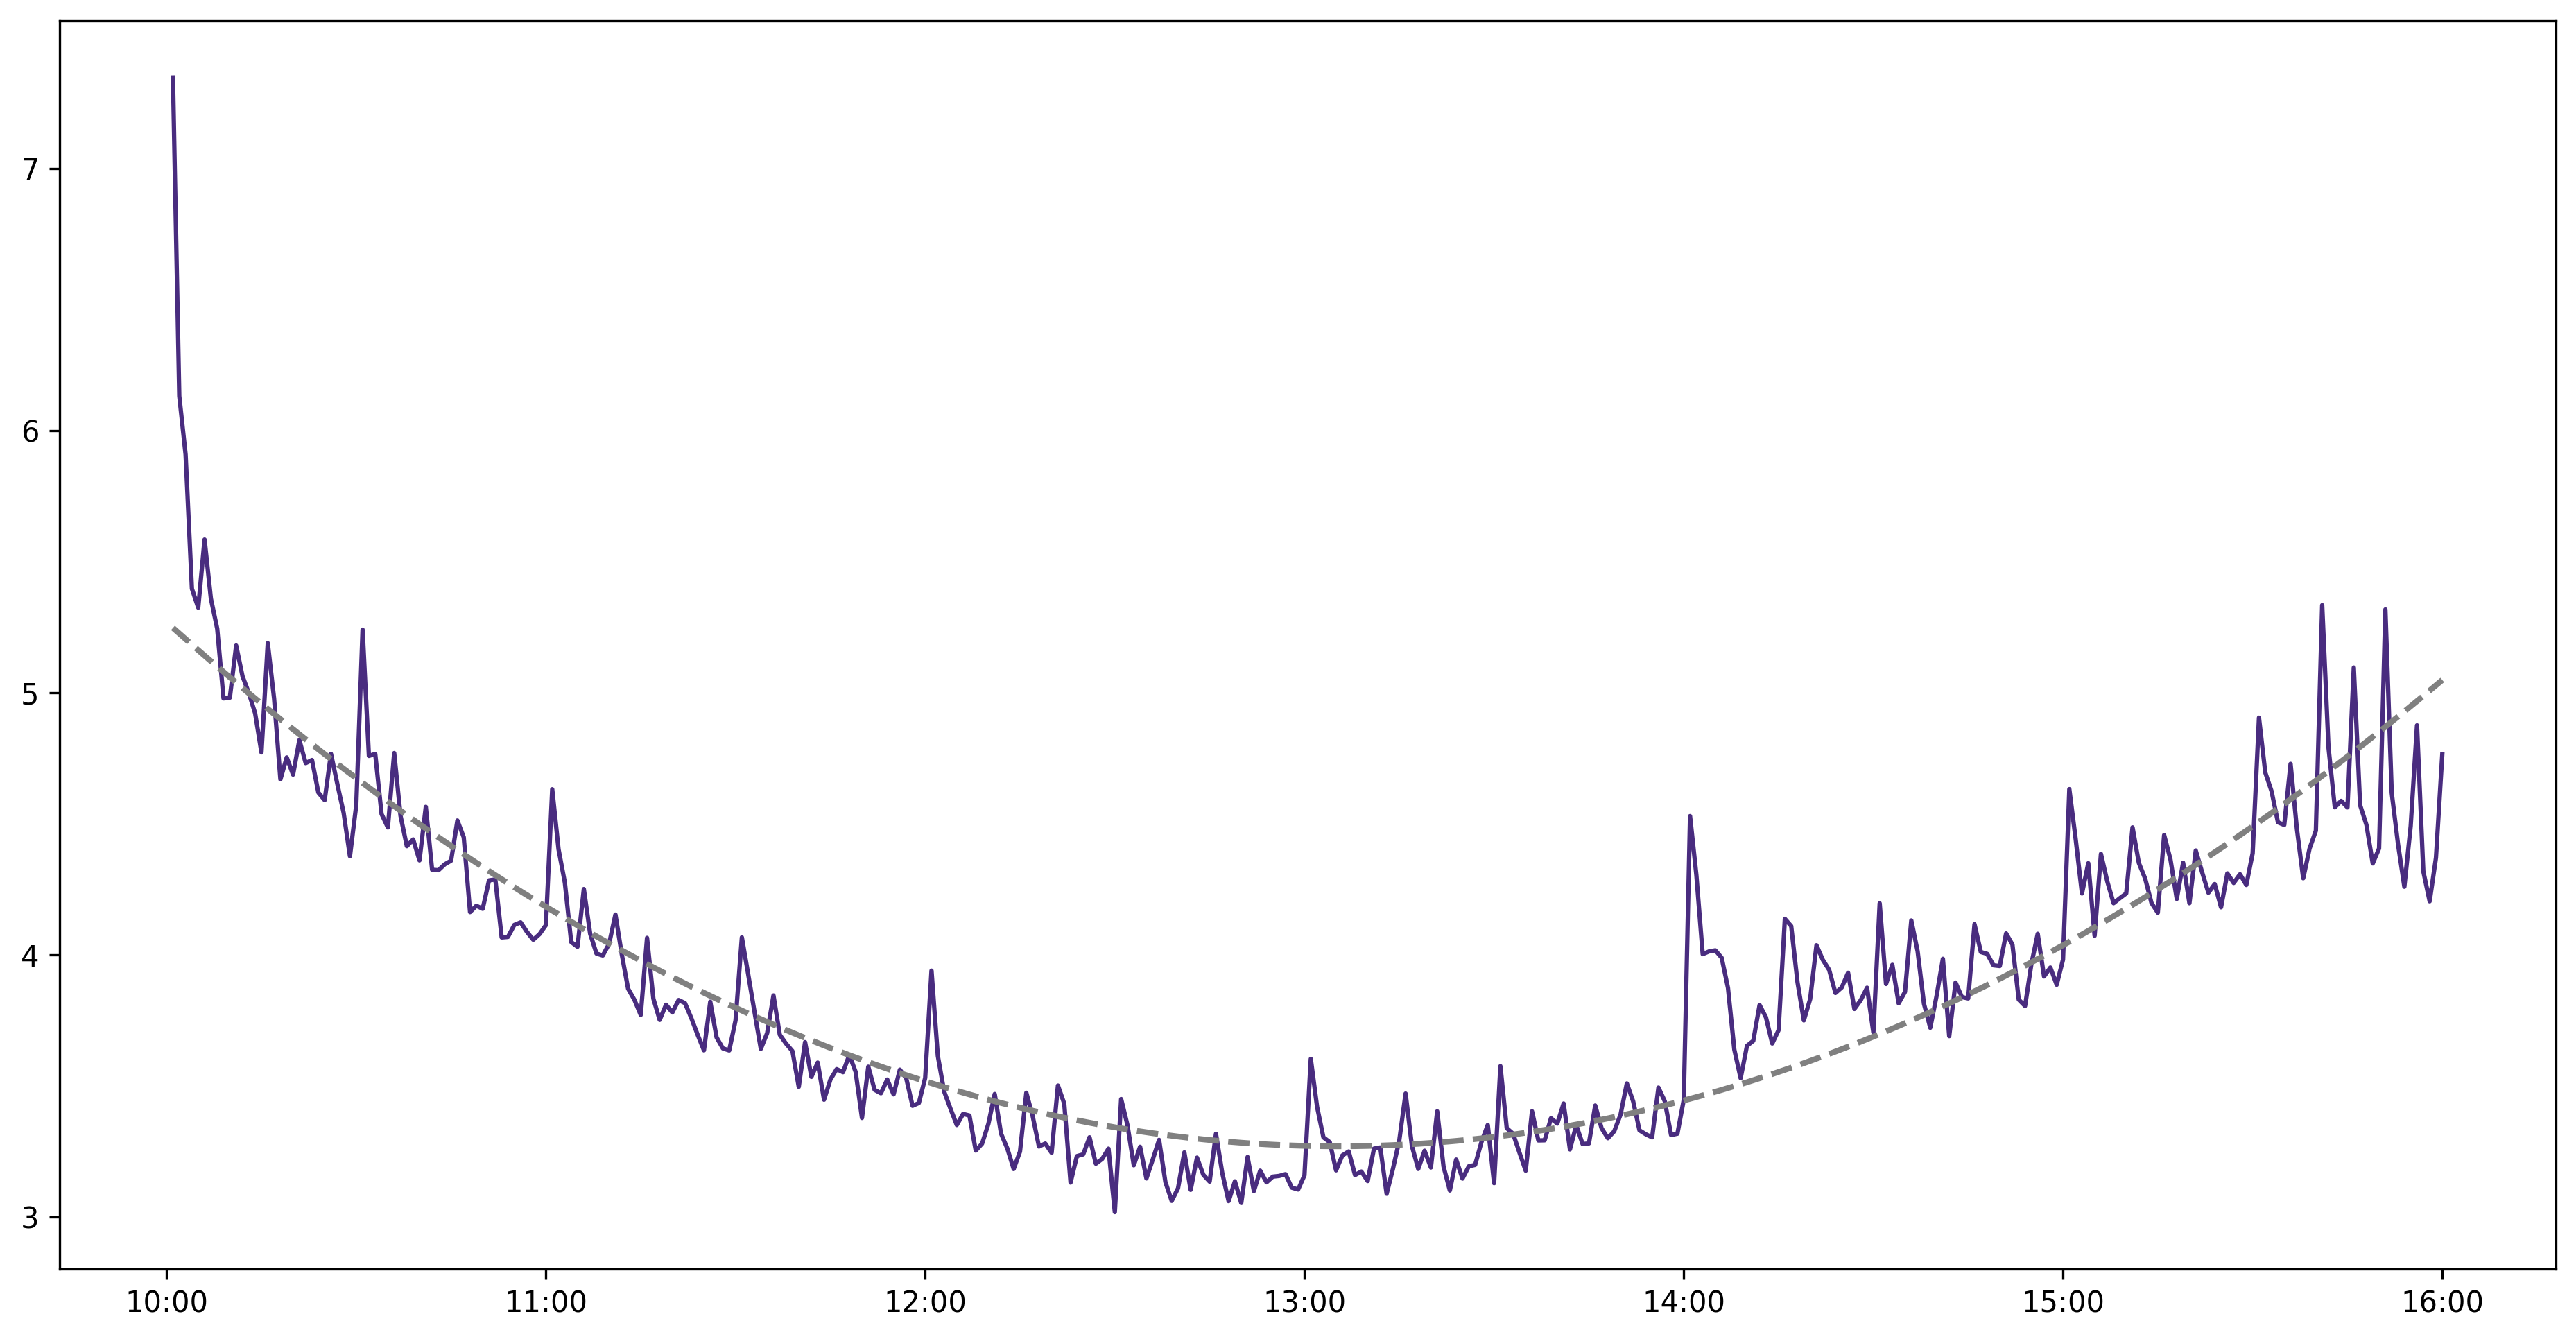
\includegraphics[width=.8\textwidth]{intraday_vol.png}
    \end{figure}

    \item We now turn to analyze how did the volatility smile changed in the last 30 years. Similar to Question 2, I plot the intraday volatility pattern for the years of 1994-1995 and 2022-2023. The results are shown in Figure~\ref{fig:volatility_smile_firstlast}. The intraday pattern is the same for both of them. 
    
    \begin{figure}[!htbp]
        \centering
        \caption{Changes in the Intraday Volatility Pattern over the years}
        \label{fig:volatility_smile_firstlast}
        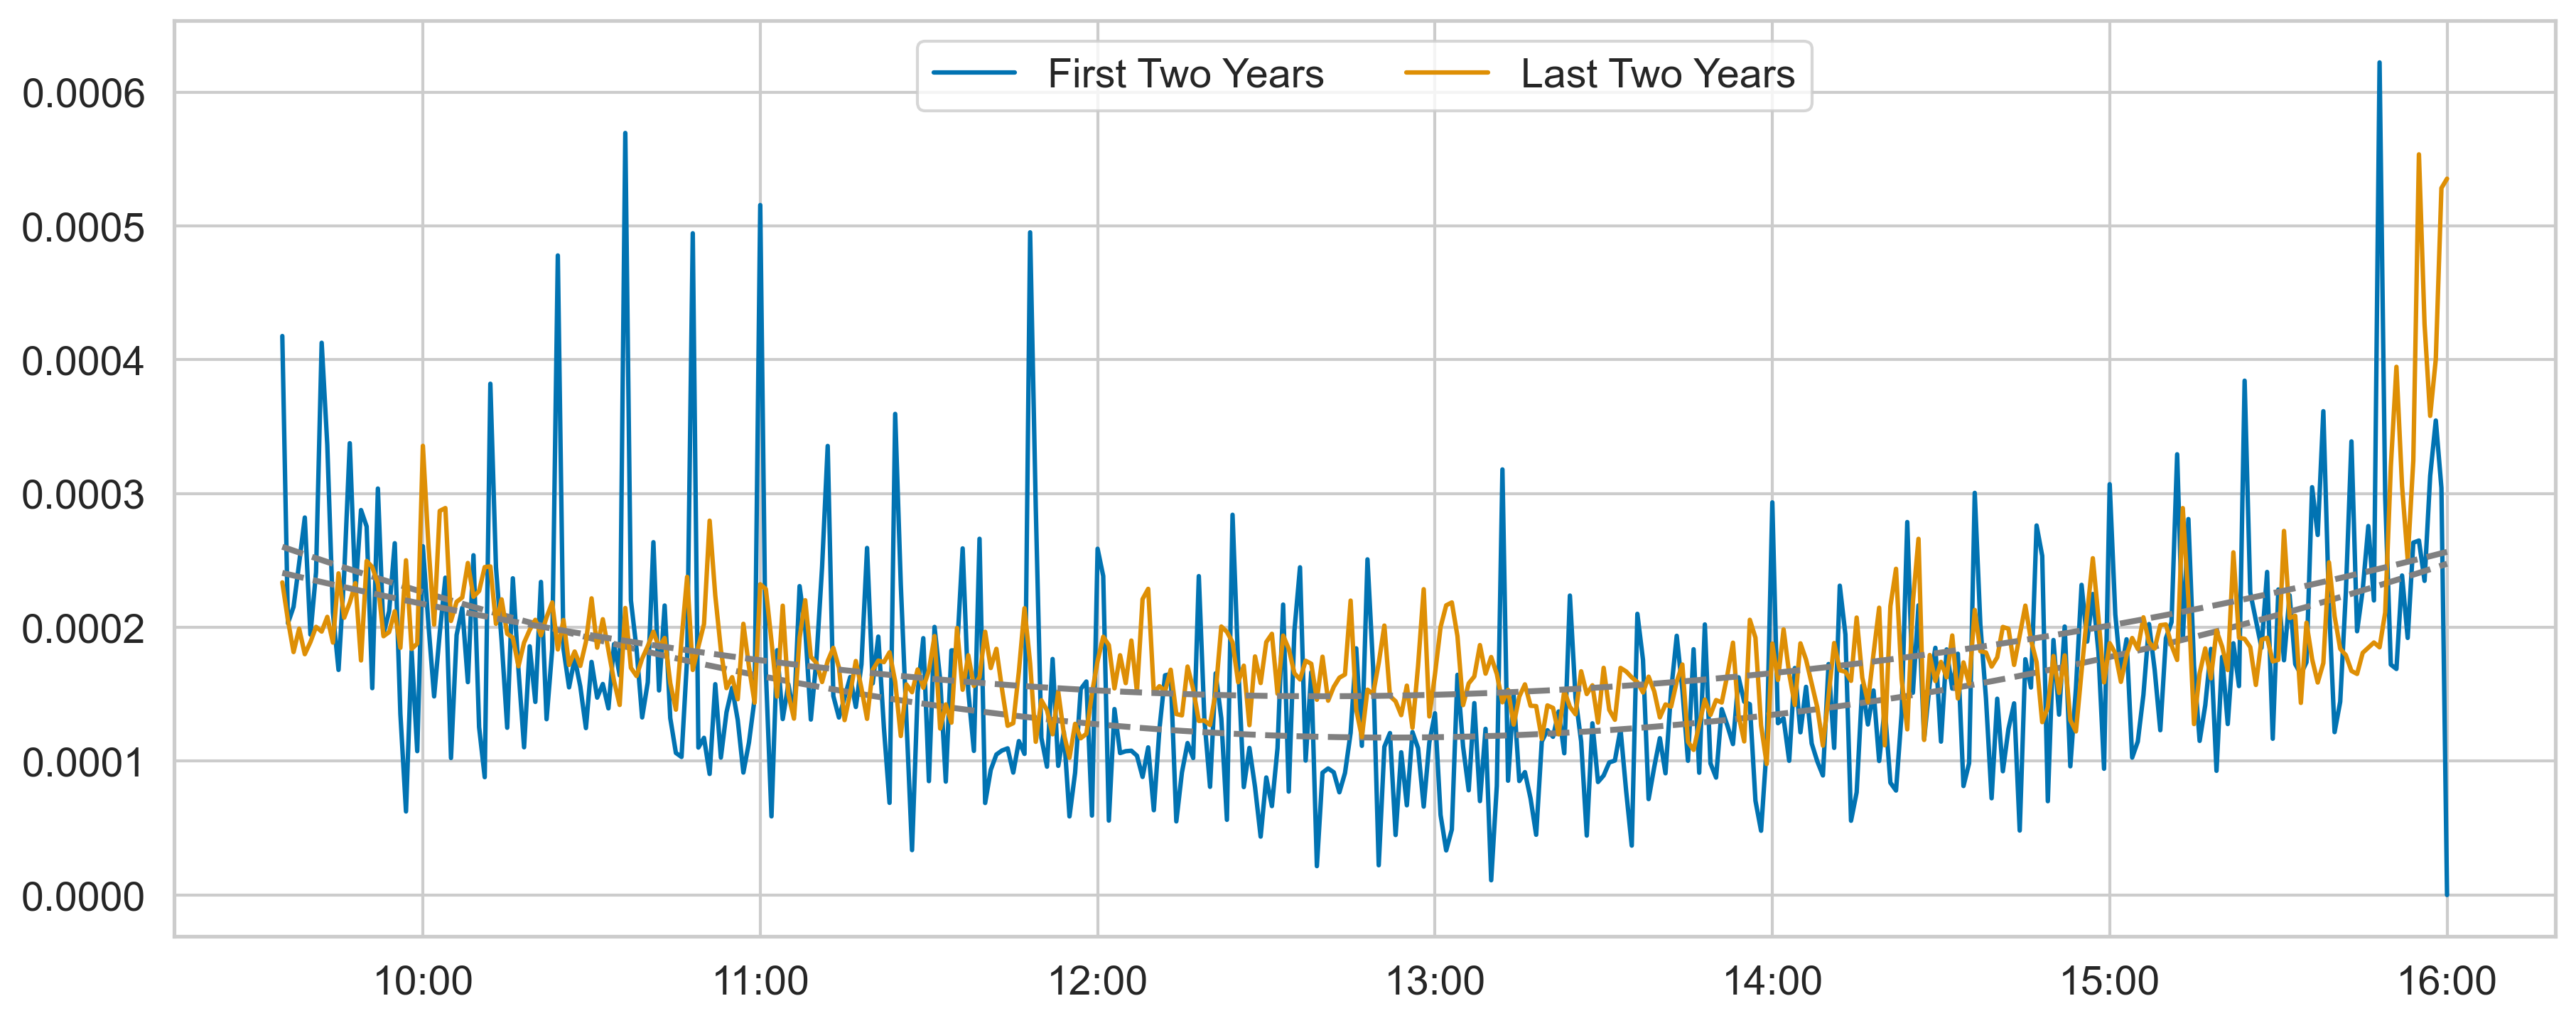
\includegraphics[width=0.8\textwidth]{intraday_vol_firstlast.png}
    \end{figure}

    \item Figure~\ref{fig:realized_volatility} displays the three measures of volatility for the full sample as well as their 30 days moving average (MA). We can see that the volatility is very high in the 2000 and 2008 crisis and in the 2019 pandemic. The volatility clusters also seem very present in our sample as higher spikes are clustered around each other. 

    In terms of persistency, Figures~\ref{fig:realized_volatility_acf} and \ref{fig:realized_volatility_pacf} show the correlogram for the three measures of volatility. We can see that the volatility is highly persistent as the ACF and PACF decay very slowly for all of them. This is consistent with the stylized fact that volatility clusters. Moreover, the log and realized volatility (squared root) seem to have a higher persistency than the regular realized variance as displayed by their longer lasting autocorrelation.
    
    \begin{figure}[!htbp]
        \centering
        \caption{Trading Day Volatility Measures}
        \label{fig:realized_volatility}
        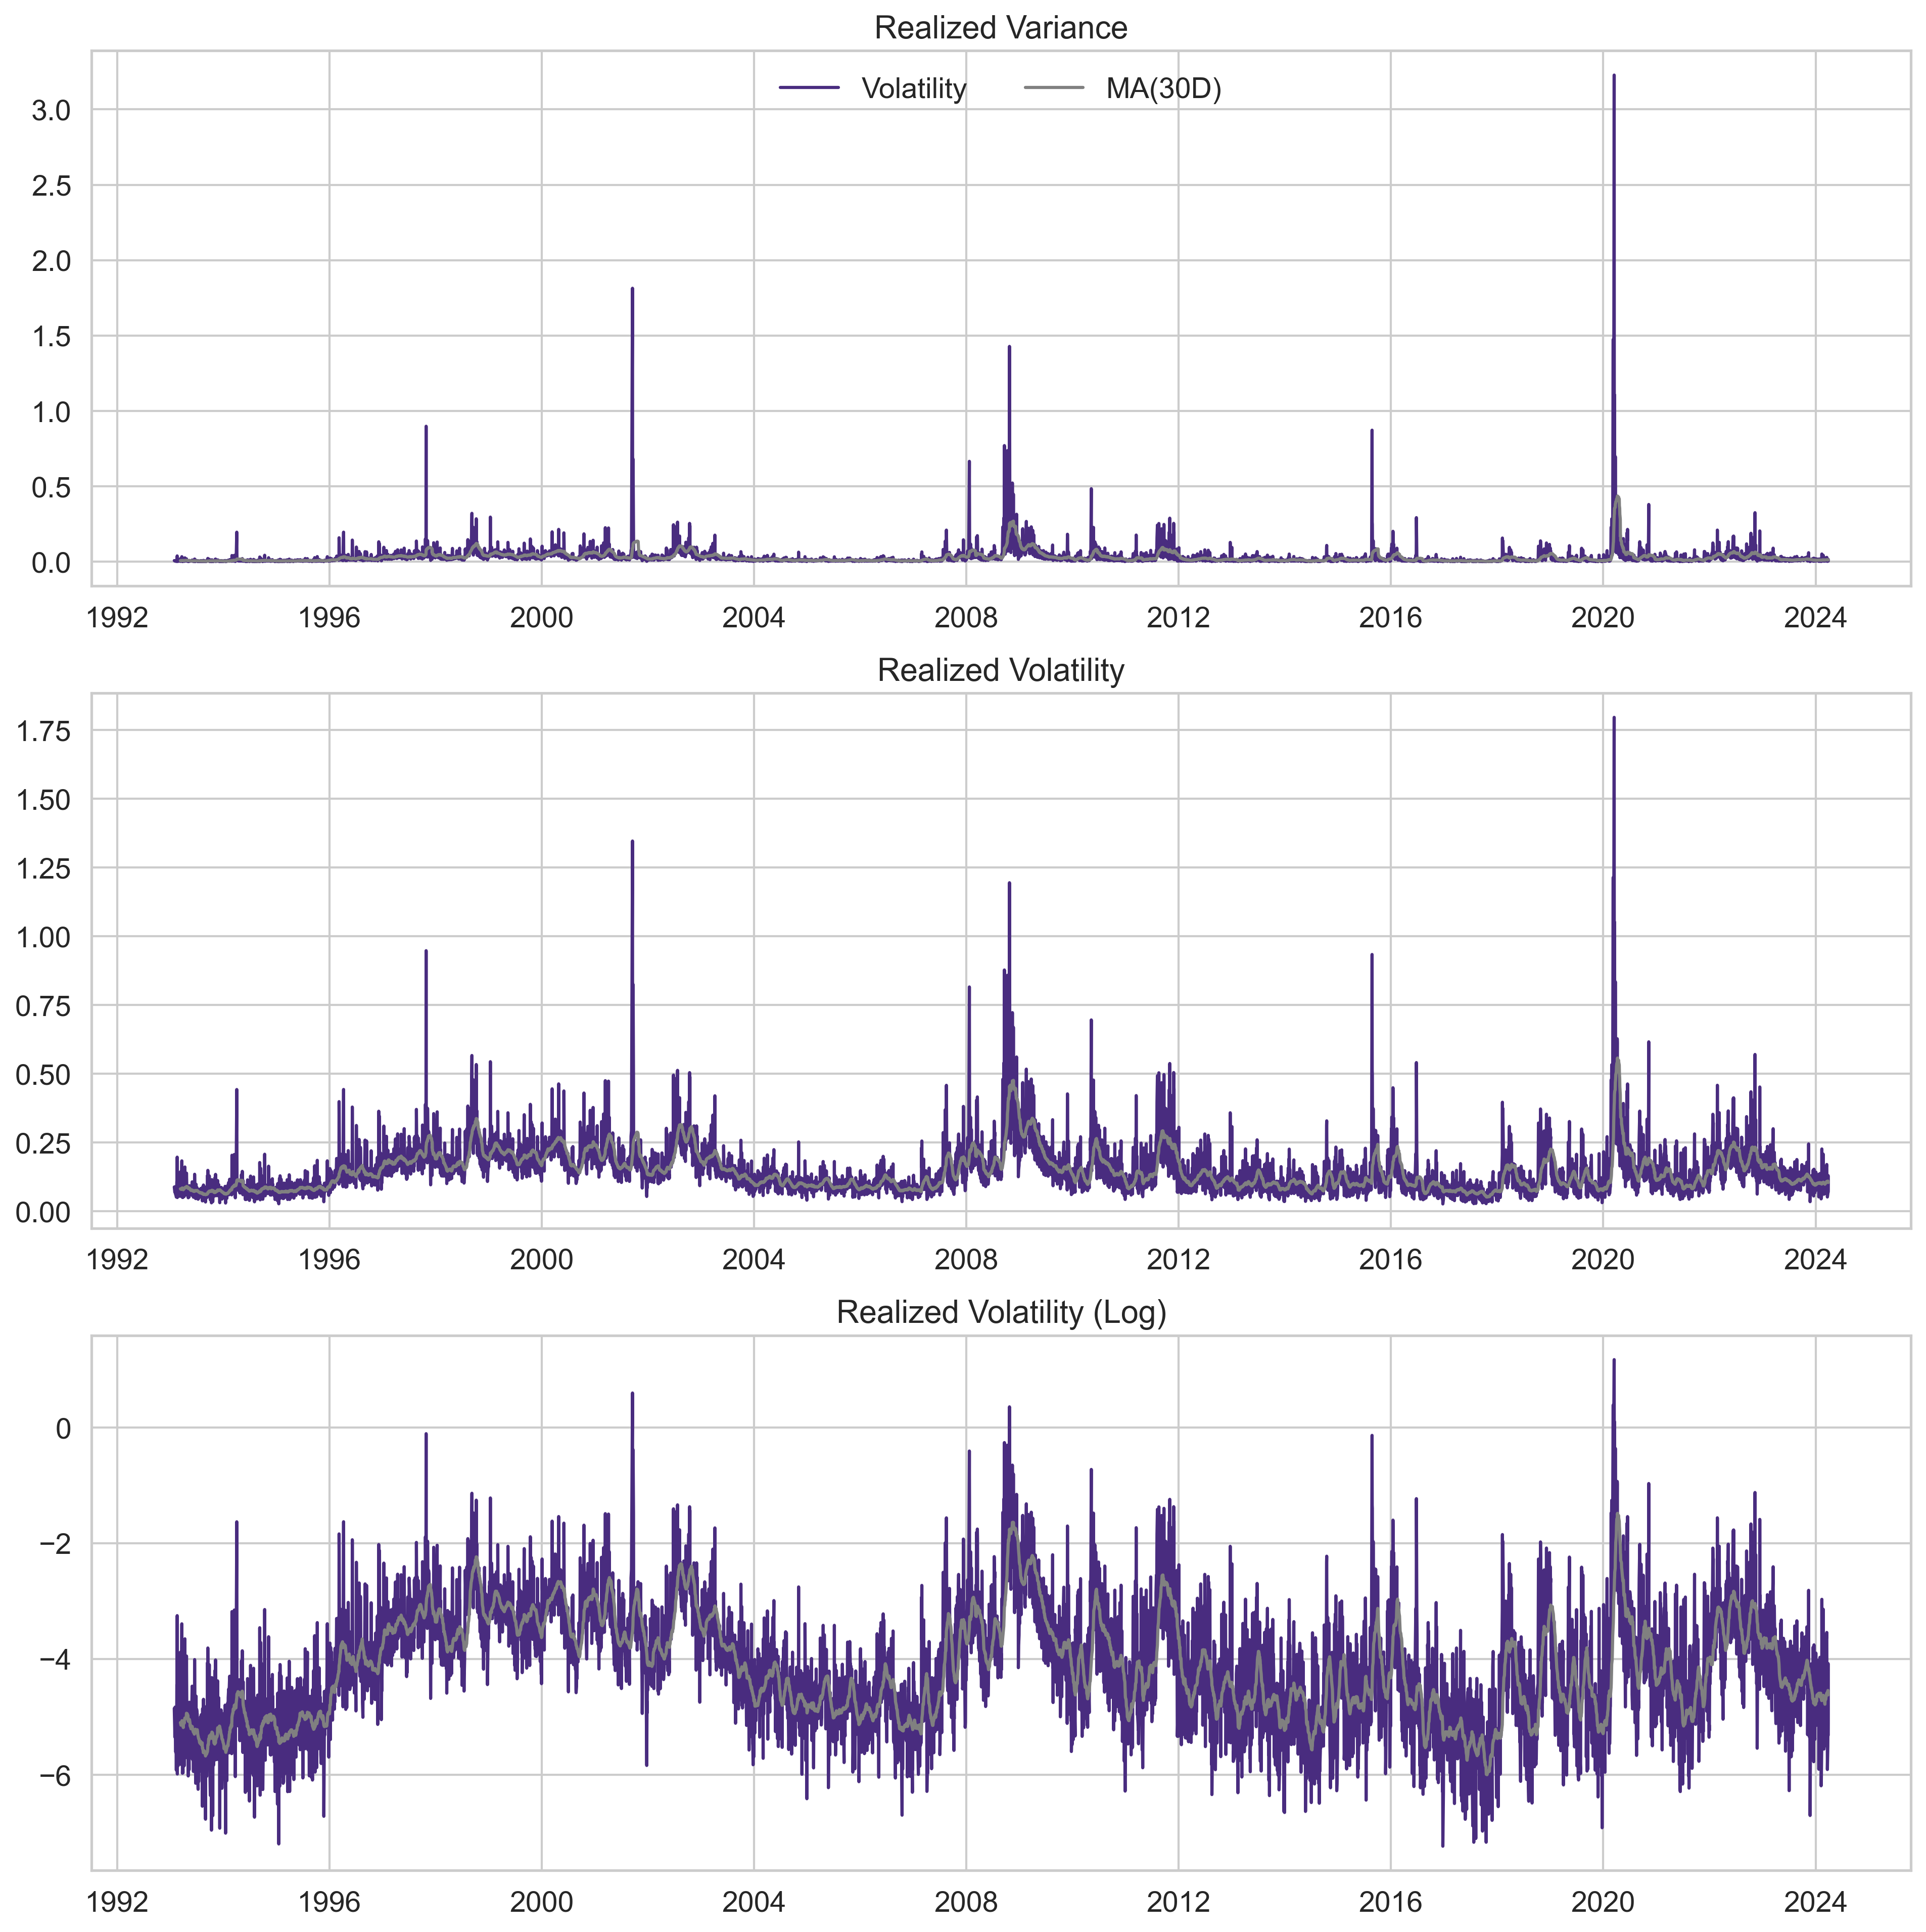
\includegraphics[width=0.8\textwidth]{realized_volatility.png}
    \end{figure}
    
    \begin{figure}[!htbp]
        \centering
        \caption{AutoCorrelation Function (ACF) of the Realized Volatility}
        \label{fig:realized_volatility_acf}
        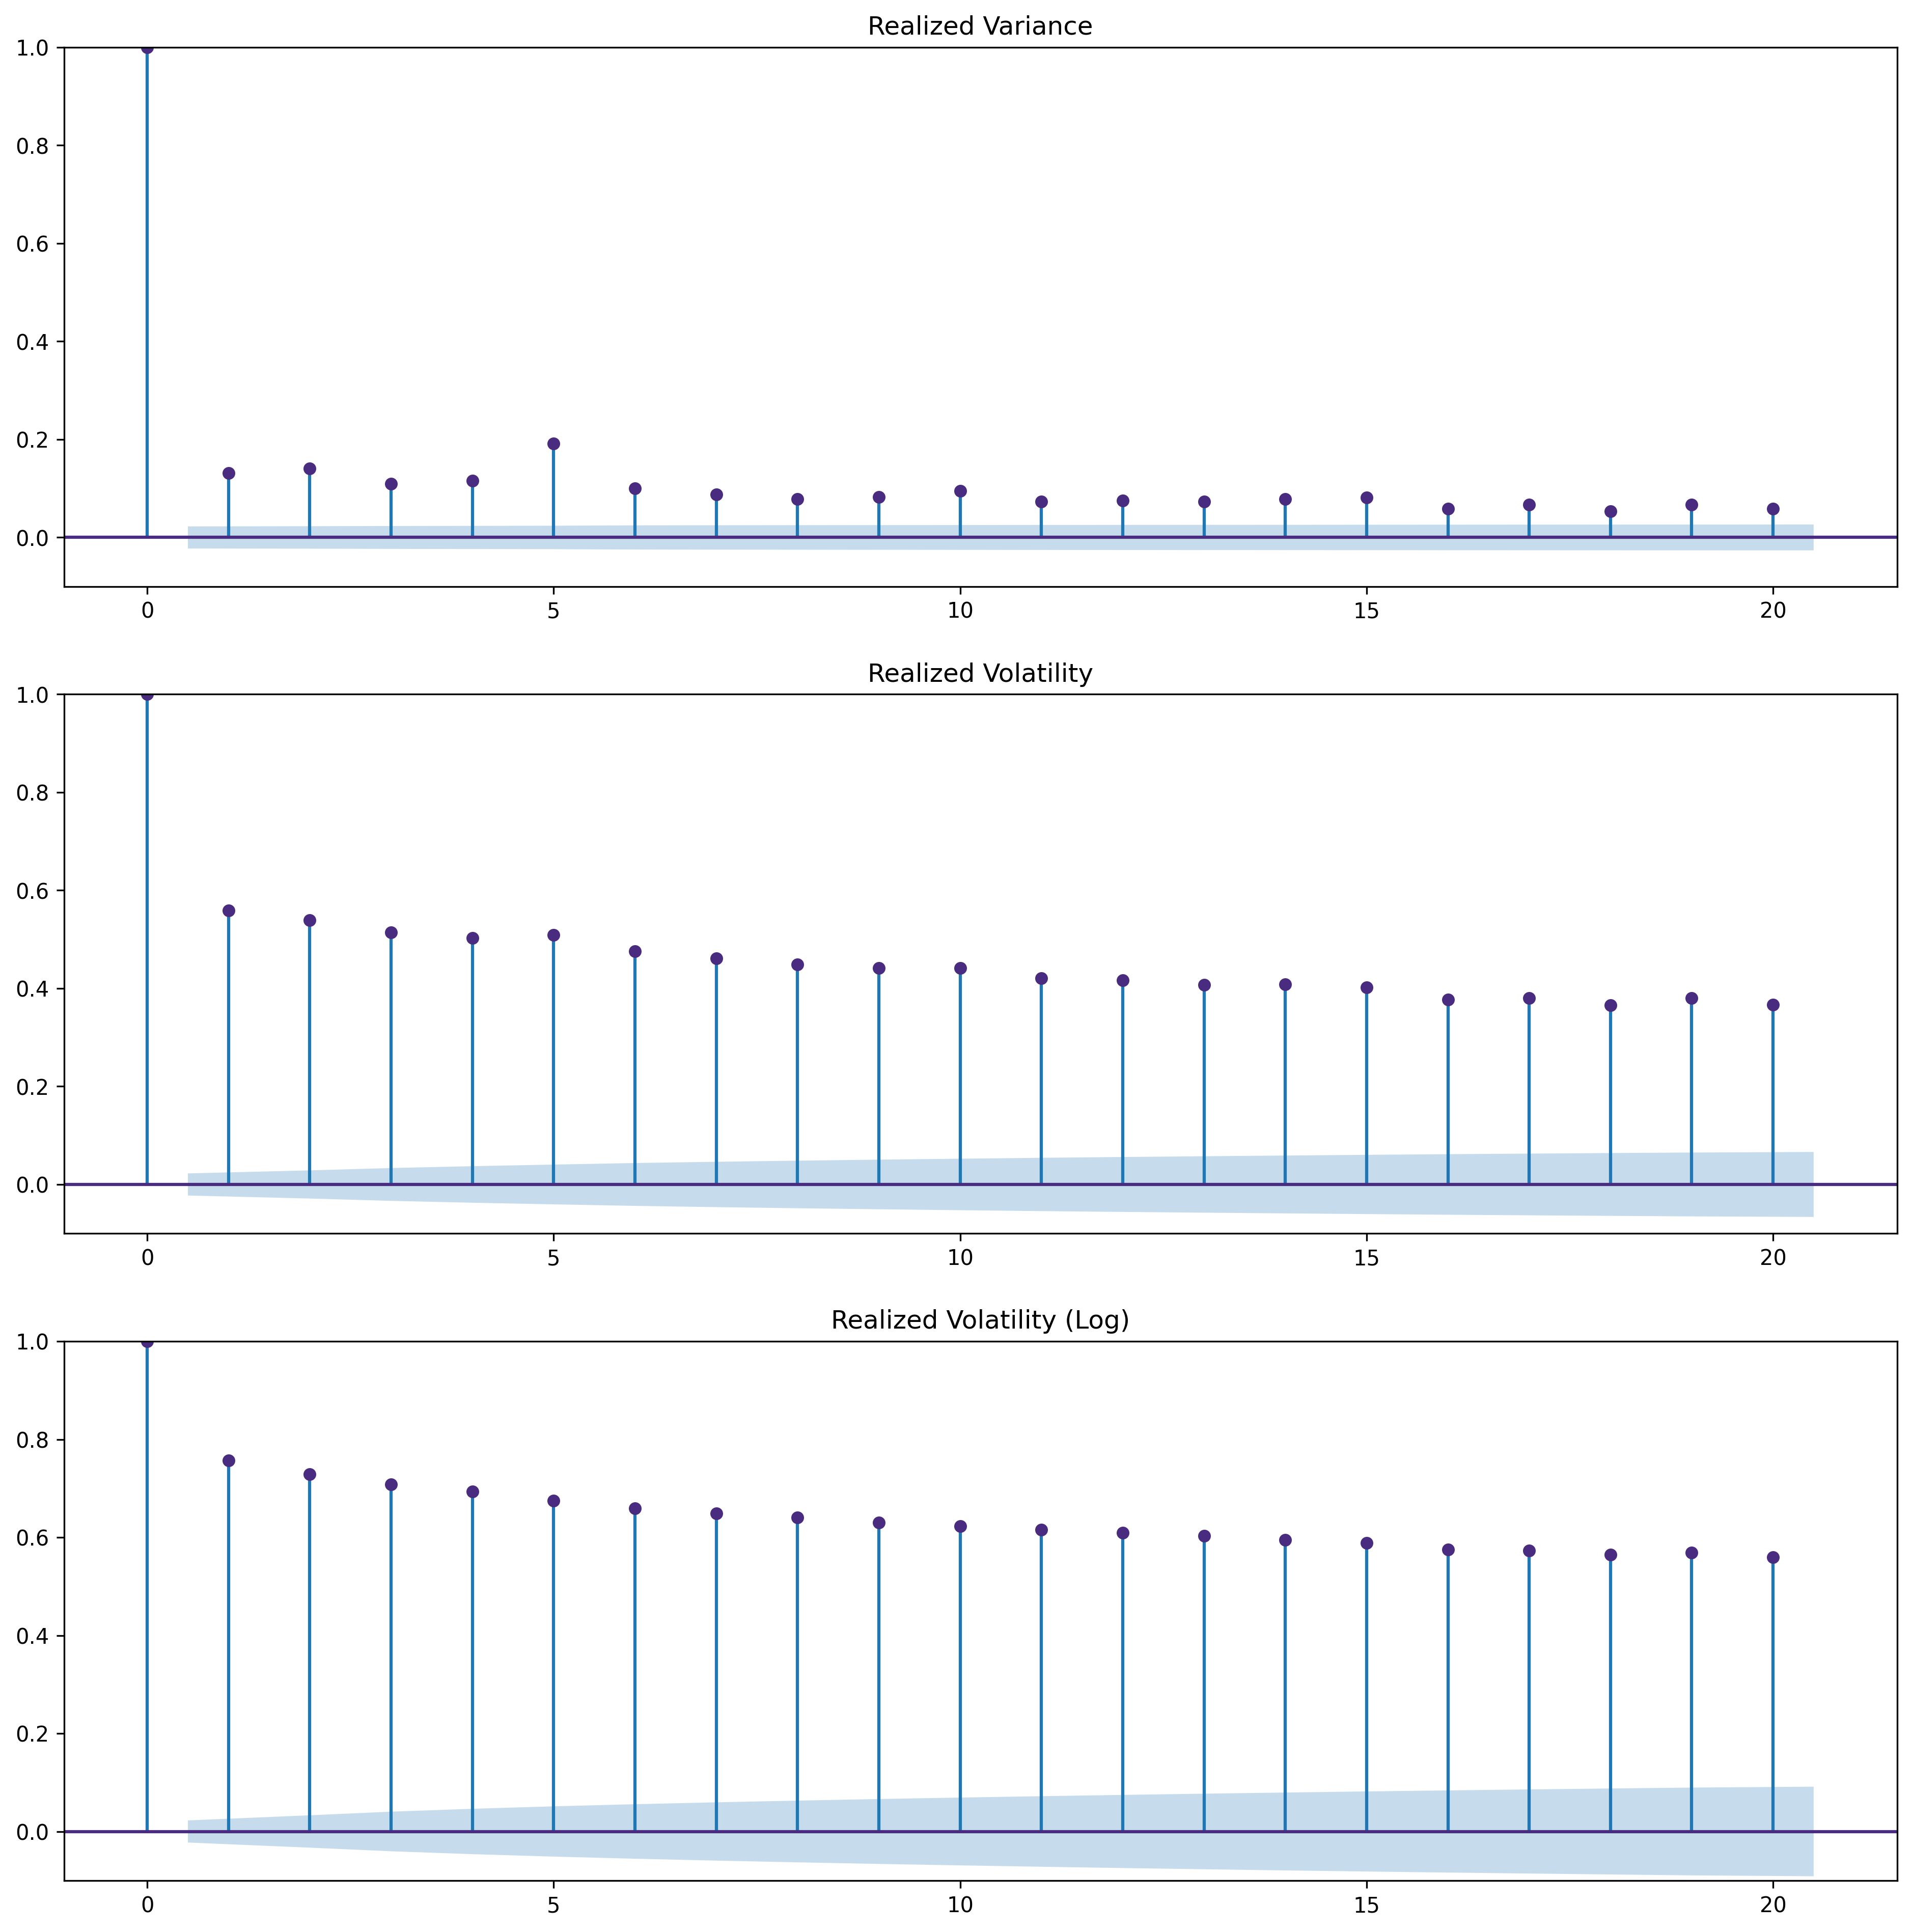
\includegraphics[width=0.8\textwidth]{realized_volatility_acf.png}
    \end{figure}
    
    \begin{figure}[!htbp]
        \centering
        \caption{Partial AutoCorrelation Function (PACF) of the Realized Volatility}
        \label{fig:realized_volatility_pacf}
        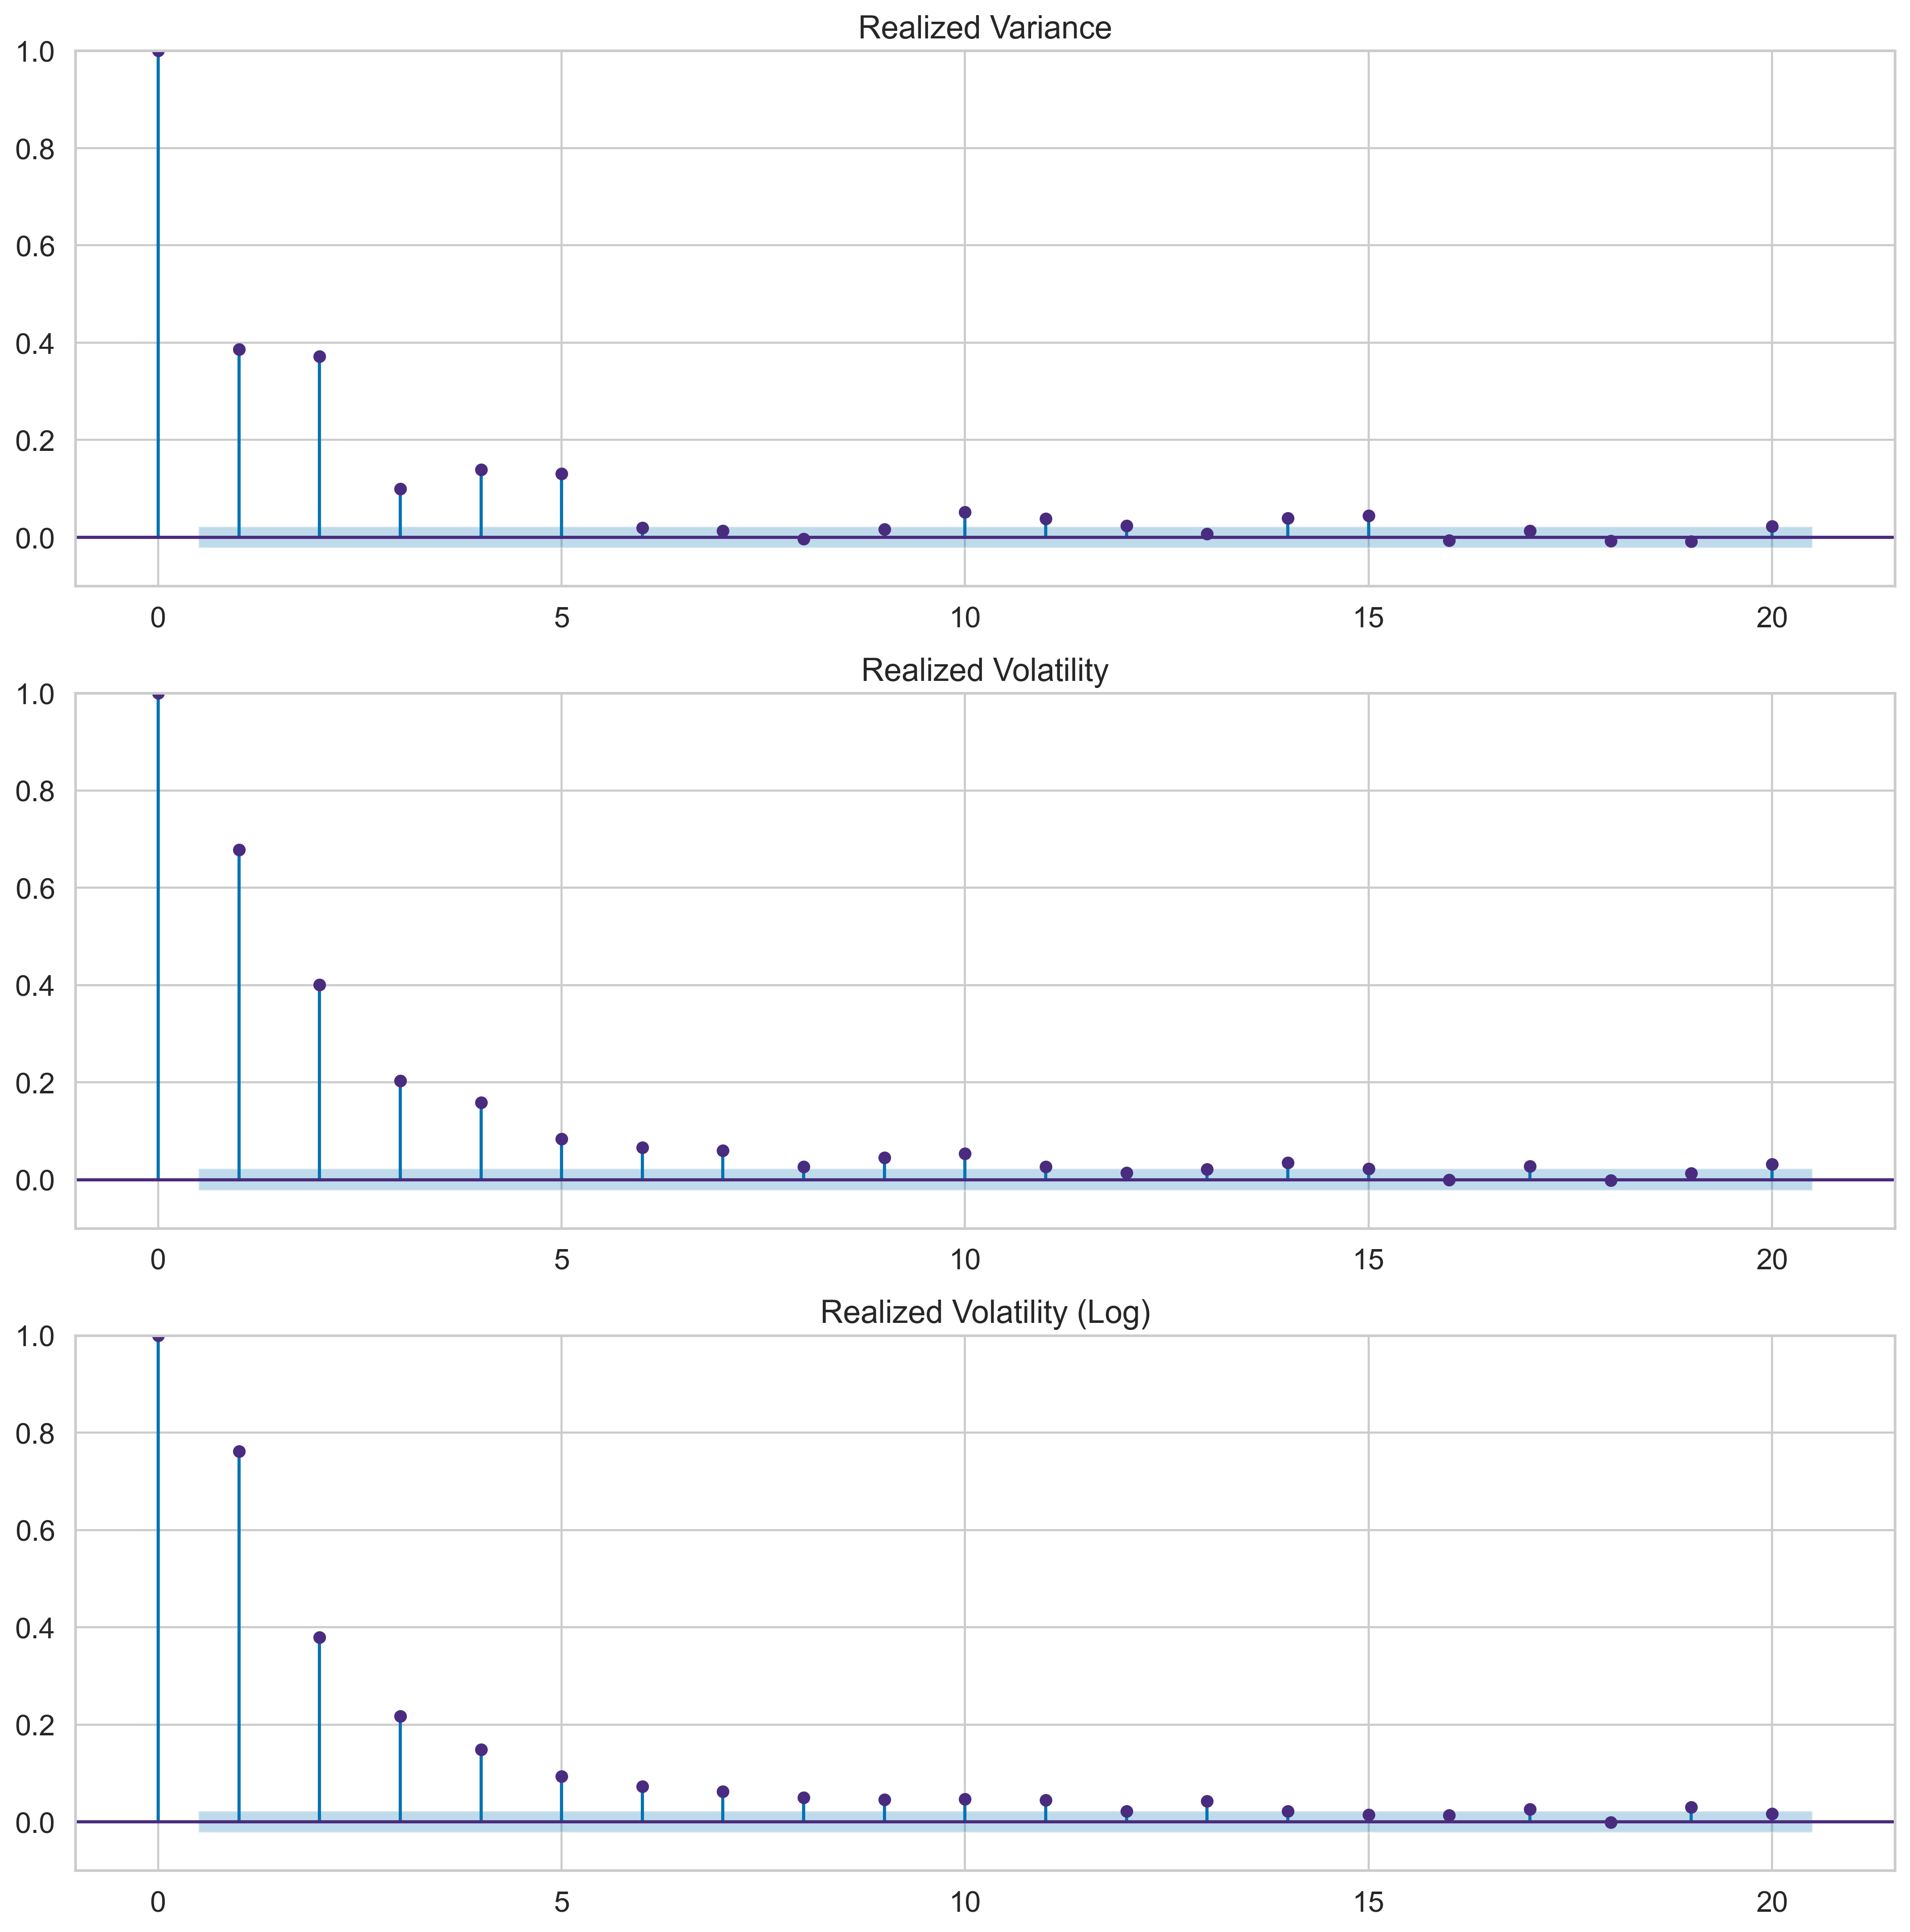
\includegraphics[width=0.8\textwidth]{realized_volatility_pacf.png}
    \end{figure}
\end{enumerate}
\end{solution}